\newpage
\section{WU10b}
We decided to work on collective classification. We use a CiteSeer dataset shared on the Statistical Relational Learning Group's webpage. (http://www.cs.umd.edu/projects/linqs/projects/lbc/index.html). The following is a description of the dataset excerpted from the webpage. \textit{The CiteSeer dataset consists of 3312 scientific publications classified into one of six classes. The citation network consists of 4732 links. Each publication in the dataset is described by a 0/1-valued word vector indicating the absence/presence of the corresponding word from the dictionary. The dictionary consists of 3703 unique words.}

We implement a stacking algorithm that is described at the end of the chapter 5 of the textbook (Algorithms 20 and 21.) We implement two flavors of the stacking algorithm (to see which one performs better):

\begin{itemize}
	\item Simple. This implementation will only use predictions on neighbors from a previous layer. (Neighbors are examples that cites/are cited by the example that we are focusing on)
	\item Cumulative. This implementation will take all the predictions on neighbors until the Kth layer $(\vec y_1, ..., \vec y_{k-1})$ to train the Kth layer's classifier.
\end{itemize}

On the first layer, we simply use Megam in our script to train a multi-class classifier. Outputs (predictions) from Megam are parsed and stored. On each succeeding layer, we first generate training data by combining original training data (training data from the first layer) with predictions from a previous layer. I.e. we append predicted labels of neighbors into the training example as features. Then we train a classifier for the layer.

We split the dataset into five parts for cross-validation and calculate training errors and test errors for each layer. For each validation step, we train classifiers with 2650 examples and test with 662 examples. 

\begin{figure}[ht]
	\begin{minipage}[b]{0.5\linewidth}
		\centering
		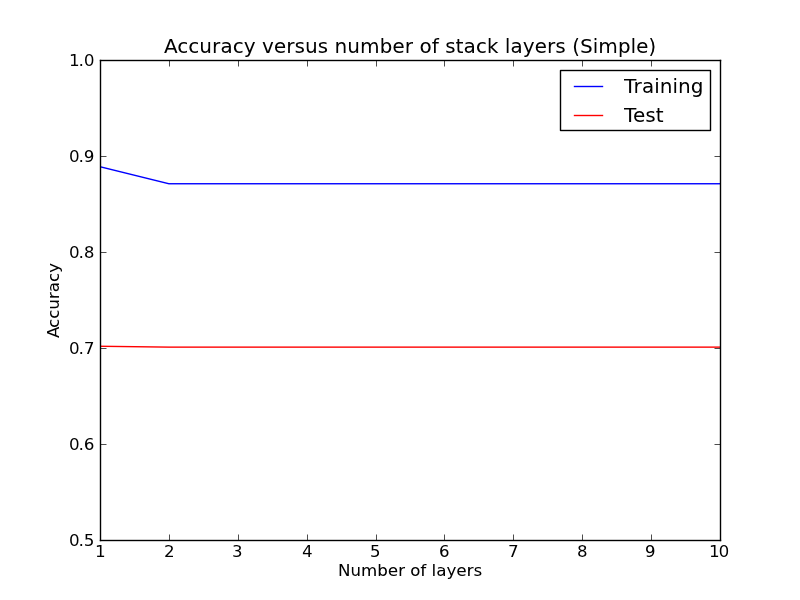
\includegraphics[width=3.2in]{images/wu10b_simple.png}
		\caption{Simple}
		\label{fig:10b_simple}
	\end{minipage}
	\hspace{0.5cm}
	\begin{minipage}[b]{0.5\linewidth}
		\centering
		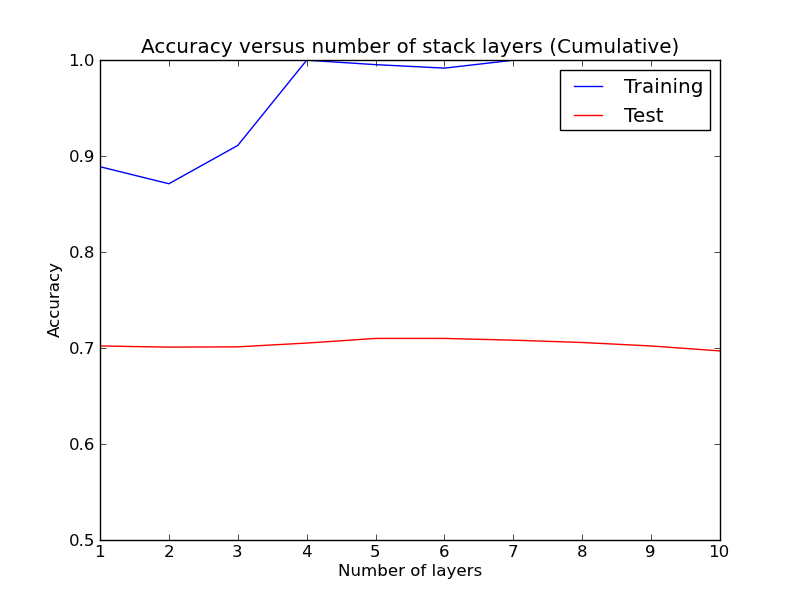
\includegraphics[width=3.2in]{images/wu10b_cumulative.png}
		\caption{Cumulative}
		\label{fig:10b_cumulative}
	\end{minipage}
\end{figure}

Figures \ref{fig:10b_simple} and \ref{fig:10b_cumulative} show training accuracies and testing accuracies against layer indexes. On the first layer of the simple implementation, training accuracy was about 89\%. The classifier is trained only with word features. On the second layer, the accuracy went down to 87\% as we append predictions from the first layer into the training dataset. The training accuracy did not change in the any of the other layers. 

The testing accuracy was 70\% on the first layer. It did not change more than 0.1\% for any of following layers.

The training accuracy on the cumulative implementation was 89\% on the first layer. On the second layer, it decreased to 87\%. After the third layer, the training error started to increase, and on the fourth layer, the training accuracy became almost 100\%. For all following layers the accuracy stayed close to 100\%.

The testing accuracy was 70\% for the first four layers. It showed a slight improvement around layer 5 and 6. There the accuracies went up to 71\%. 

Both simple and cumulative implementations of the stacking algorithm did not show a significant improvement in test accuracy. We believe there are several reasons for this behavior:
\begin{itemize}
	\item Dataset's network is sparse. There are more word features compared to neighbor features. Therefore neighbors' labels are less influential for classification.
	\item Neighbors' labels do not contain much information. Collective classification assumes neighbors' labels are informative because ML papers are more likely cited by other ML papers. However, in this dataset, AI paper can certainly cite ML papers, and so for others.
\end{itemize}

We implemented a program for collective classification with two flavors of the stacking algorithm. We used CiteSeer dataset which consists of scientific publications classified into one of six classes. The performance in the simple implementation of the stacking algorithm did not improve. The performance in the cumulative implementation improved at layers 5 and 6 compared to the first layer, but only by 1\%. We believe the reason why the accuracy did not show significant improvement is because of the sparse network. Collective classification would be more effective if the vertices are more densely connected to each other so neighbors' labels are more influential.